\documentclass[conference]{IEEEtran}
\IEEEoverridecommandlockouts
% The preceding line is only needed to identify funding in the first footnote. If that is unneeded, please comment it out.
\usepackage{cite}
\usepackage{amsmath,amssymb,amsfonts}
\usepackage{algorithmic}
\usepackage{graphicx}
\usepackage{textcomp}
\usepackage{url}
\usepackage{multicol}

\usepackage[dvipsnames]{xcolor}
\newcommand{\todo}[1]{\textcolor{red}{\emph{Todo: #1}}}

\begin{document}

\title{Integrated C-ITS Reference Architecture* \\
  {\footnotesize \textsuperscript{*}Industrial Experience Report}
  \thanks{Funded by European Union Commission , 723311.}
}

\author{
  \IEEEauthorblockN{Priyanka Karkhanis,
    Mark van den Brand, Saurab Rajkarnikar}
  \IEEEauthorblockA{Eindhoven University of Technology\\
    Eindhoven, The Netherlands\\
    Email: p.d.karkhanis@tue.nl,
    M.G.J.v.d.Brand@tue.nl,
    s.rajkarnikar@tue.nl}
}

\maketitle


\begin{abstract}
C-ITS (Cooperative Intelligent Transport Systems) aims to facilitate cooperative, connected and automated mobility.
It is based on the concept of System of Systems and promotes a new way of thinking for solving grand challenges where the interactions of technology, policy and economics are the primary drivers.

The C-ITS domain comprises widely spread systems like traffic management systems, traffic light controllers, and vehicle on-board units. Such complex and heterogeneous systems have independent uses but demand a strategy to facilitate their convergence.

C-ITS is currently demonstrated by ongoing project C-MobILE (Accelerating C-ITS Mobility Innovation and depLoyment in Europe) which is a large scale demonstration project spanning from 2017-2020.

The main objective of C-MobILE is to define an integrated architecture based on a number of existing C-ITS projects.
The architecture provides a way to standardize and a unifying modeling approach by means of a common language that can be reused by other organizations to guide their internal development processes.

The ref. arch. is defined using the C-ITS arch. framework that is compatible with the ISO/IEC/IEEE 42010 \cite{iso42010} international standard for architecture descriptions of systems.
In this paper, we present the C-MobILE C-ITS reference architecture that is aimed at large scale deployment and demonstration with partner deployment sites across Europe and share the lessons learned during the process.
\end{abstract}

\begin{IEEEkeywords}
C-ITS, ITS, Architecture Framework, transportation
\end{IEEEkeywords}


\section{Introduction} -

The European Parliament in its directive 2010/40/EU \cite{ec} defines Intelligent Transport Systems (ITS) as "systems in which information and communication technologies are applied in the field of road transport, including infrastructure, vehicles and users, and in traffic management and mobility management, as well as for interfaces with other modes of transport."
ITS can be further described as systems which aim to make transportation safe and economical by combining data from the vehicles and other sensors on the roadway together with weather information. It began during the 1990s\cite{itsbegin} with projects in
\begin{itemize}
	\item the US (named Intelligent Vehicle Highway System \cite{ivhs})
	\item various countries in Europe (with the program Prometheus \cite{prometheus})
	\item Japan (with a research committee Road/Automobile Communication System \cite{racs})
\end{itemize}

Cooperative-Intelligent Transport Systems (C-ITS) \cite{c-its} adds upon ITS by providing ways for connected vehicles to interact with other connected vehicles or any infrastructure such as the traffic light controller, roadway signals or roadside units. This interaction is where the term cooperatives comes from. In this scenario the vehicles can act as sensors as well.

The C-ITS domain covers not only the field of software- and systems engineering, but also traffic engineering, civil engineering, and information technology, which require a unified architecture for the C-ITS domain.

C-ITS is currently demonstrated by ongoing project C-MobILE (Accelerating C-ITS Mobility Innovation and depLoyment in Europe) which is a large scale demonstration project from 2017-2020. The C-MobILE aims for a fully safe and efficient road transport without casualties and serious injuries on European roads.
 
The C-MobILE project is an EU project that spans across eight C-ITS equipped deployment sites and regions with more than 37 participating institutes and companies. 
The C-ITS equipped deployment sites partnering with C-MobILE are:

\begin{table}[ht!]
	\centering
	\begin{tabular}{ll}
	1. Newcastle, UK	& 2. Bordeaux, France \\
	3. North Brabant, the Netherlands	& 4. Vigo, Spain \\
	5. Bilbao, Spain	& 6. Barcelona, Spain\\
	7.  Thessaloniki, Greece	& 8. Copenhagen, Denmark  
	
	\end{tabular}
\end{table}

There are 20 C-ITS services, such as Road Hazard Warning, Road Works Warning and Green Light Optimal Speed Advisory considered for the C-MobILE project.

The architecture definition process in C-MobILE has been defined to support the following sub-goals.


\begin{itemize}
  \item Analyse existing C-ITS architectures to provide common concepts and vocabulary.
  \item Create a reference architecture that enables pan-European interoperability of C-ITS  architectures based on the generalization of existing C-ITS architectures.
\end{itemize}

In this paper, we share the C-MobILE C-ITS reference architecture, which is a result of the first six months of the project.

\section{Related Works}
There are various existing and ongoing C-ITS projects . Of those projects, the following were reference architecture projects.\todo{fix the sentence}

\begin{enumerate}
	\item Dutch C-ITS Reference Architecture (DITCM)\cite{ditcm}\cite{ditcmits}:\\
		This project focused mostly in developing a reference architecture for large scale C-ITS deployment in the Netherlands. It was build based on current and some finished C-ITS projects.
	\item CONVERGE\footnote{\label{converge}Converge. \url{https://converge-online.de/}}: \\
		This was a German funded project that developed an open platform for service providers with focus on Car2X (V2X or Vehicle to Vehicle/Infrastructure) Systems Network.
	\item COMPASS4D\footnote{\label{compass4d}Compass4d. \url{http://ertico.com/projects/compass4d/}.}:\\
	This was an EU funded project that worked with three C-ITS services such as Road Hazard Warning, Red Light Violation Warning and Energy Efficiency Intersection Service.
	\item NordicWay\footnote{\label{nordicway}Nordicway.\url{http://vejdirektoratet.dk/EN/roadsector/Nordicway/Pages/Default.aspx}.}:\\
	This project, as the name suggests, focused mostly on the Nordic countries (Finland, Sweden, Norway and Denmark) and is a pre-deployment pilot project for  C-ITS deployment.
	\item US-ITS (ARC-IT)\footnote{\label{arcit}Arc-it version 8.1. \url{https://local.iteris.com/arc-it/}}:\\
	The US-ITS or ARC-IT project is a large scale reference architecture that acts as building blocks for small scale regional C-ITS projects in various regions of the USA.

\end{enumerate}

These reference architecture projects defined their own multidisciplinary approach towards their deployed strategy. 

The Dutch C-ITS Reference Architecture used standard notations which considered the requirements for the Netherlands and CONVERGE  for Germany while the US-ITS project used their own notations. Projects such as NordicWay and Compass4D did not focus on many services, rendering those projects unsuitable for large scale deployment across Europe.

\section{Problem Statement}
As described in the related project section, 
the existing C-ITS projects had their own ad-hoc notations that creates inconsistencies towards achieving the goal of developing a base for large scale C-ITS deployments.

In addition, the partner deployment sites have their own C-ITS implementations with their own C-ITS architecture, ad-hoc notations and differing categorizations.

Thus, there is no standard notation for use in a large scale deployment, to the best of our knowledge. This demands a standardized approach to consolidate and integrate existing architectures, addressing concerns such as security and maintainability.

This is where the C-MobILE project comes in. It aims for a large scale demonstration across various deployment sites with an architecture that harmonizes existing technologies without changing the existing architectures. It also plans to be a building block or the base for future C-ITS implementations in other cities or regions.

\section{Methodology}
The term "Reference Architecture" has various meanings, multiple purposes and uses, varying levels of detail and abstraction, and very little common guidance. However, for C-ITS a reference architecture provides a common vocabulary with which to discuss implementation, often with the aim to stress commonality often based on the generalizations of a set of solutions. 

To develop a common and compatible reference architecture, we analysed existing C-ITS reference architectures and projects that included the Dutch C-ITS Reference Architecture (DITCM) \cite{ditcm}\cite{ditcmits}, CONVERGE\footnotemark[\ref{converge}], COMPASS4D\footnotemark[\ref{compass4d}], MOBiNET\footnote{\label{mobinet}MOBiNET. \url{http://www.mobinet.eu/}}, NordicWay\footnotemark[\ref{nordicway}], SCOOP@F\footnote{SCOOP@F. \url{https://ec.europa.eu/inea/en/connecting-europe-facility/cef-transport/projects-by-country/multi-country/2014-eu-ta-0669-s}}, and US-ITS (ARC-IT)\footnotemark[\ref{arcit}].

Besides these C-ITS architectures, we considered ITS implementations of the deployment sites involved with C-MobILE.

For the definition of the reference architecture, we used the C-ITS architecture framework which is defined in the scope of the C-MobILE project. We extracted the systems, components, protocols, networks, and technology details from these architectures manually, as illustrated in Figure \ref{methodology} \cite{d31}.
The C-ITS architecture framework is based on the ISO/IEC/IEEE 42010 \cite{iso42010} international standard for architecture descriptions of systems and software \cite{sysml} and uses architecture viewpoints of the architecture framework for automotive systems \cite{dajsuren2015design}.

\begin{figure}[ht!]
	\centering
	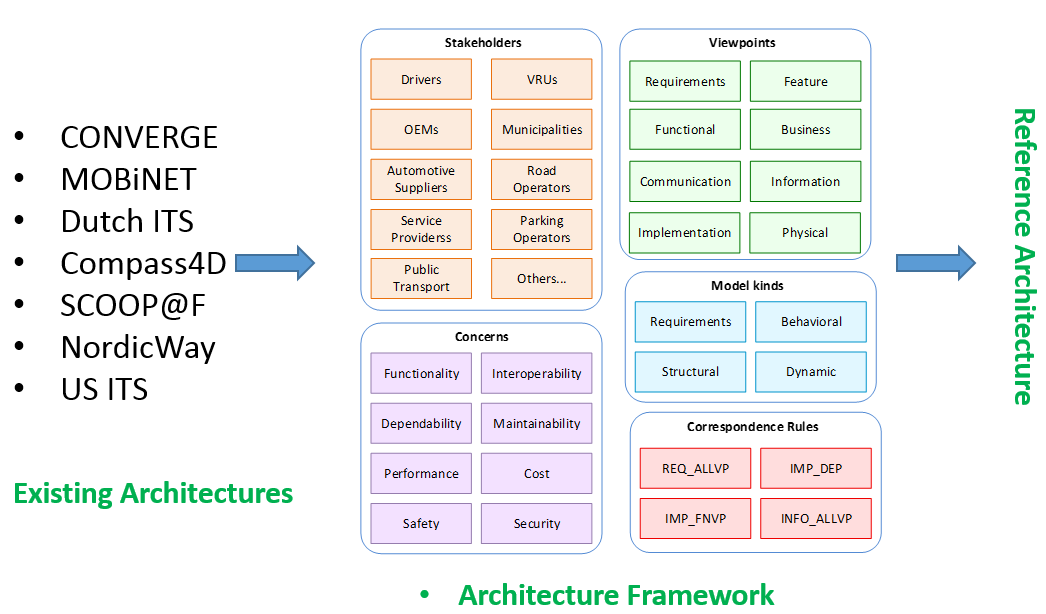
\includegraphics[width=0.47\textwidth]{methodology}
	\caption{Developing a reference architecture for C-ITS by extracting and reverse engineering of existing architectures}
	\label{methodology}
	\centering
\end{figure}

To describe the reference architecture, Systems Modeling Language (SysML) was used. SysML is a general purpose modeling language for engineering systems, and consist of structure diagrams, requirement diagrams and behavior diagrams. Having a common architecture framework and modeling language, enables the C-ITS organizations to guide their internal process as it reflects a common understanding of C-ITS.

In the following section, we present the reference architecture.

\section{C-MobILE Reference Architecture}
\label{secCMobILEReferenceArchitecture}

The C-MobILE Reference Architecture describes various systems at a high level in the form of models using SysML structural diagrams, providing high level information to architects and other stakeholders.

The C-MobILE project neither has the resources nor the intention to redefine all those standards.
Instead, at high level we highlight the common systems, their interfaces and protocols by considering various existing projects to ensure interoperability.

As a result of the architecture analysis, we have extracted the reference architecture from various existing architectures, which was consistent with the DITCM reference architecture \cite{ditcm}\cite{ditcmits}. As an illustration of the reference architecture, we discuss here the context and functional views by displaying the context model representation in Figure \ref{fig:contextviewpoint} and the functional model representation in Figure \ref{fig:functional}. 

The system structure is captured by categorizing into systems such as Central, Roadside, Vehicle and Traveler/VRU System with a Support System that supports all the other systems (Figures \ref{fig:contextviewpoint} and \ref{fig:functional}). Here, VRU means Vulnerable Road User such as a pedestrian or a cyclist. These systems are further decomposed into subsystems such as Traffic Management System (TMS) for the Central System as illustrated in Figure \ref{fig:functional}.

\begin{figure}[ht!]
	\centering
	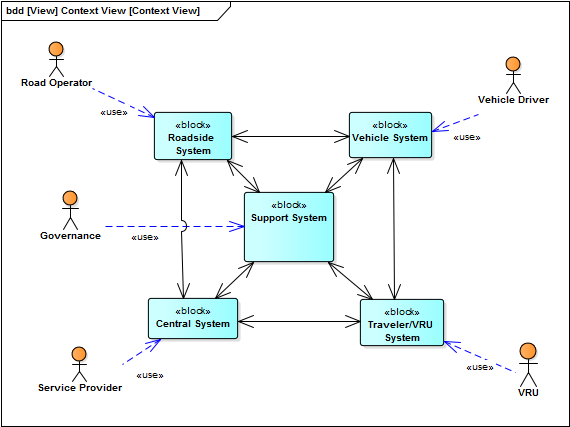
\includegraphics[width=0.45\textwidth]{context}
	\caption{Context Model Representation of the C-MobILE Reference Architecture}
	\label{fig:contextviewpoint}
	\centering
\end{figure}
The context viewpoint describes the relationships, dependencies, and interactions between the system and its environment (e.g. people,
systems and external entities) \cite{sysml}. The context view (Figure \ref{fig:contextviewpoint}) conforms to the context viewpoint and helps system’s stakeholders (e.g. system/software architects, designers, developer and users) understand the system context \cite{d31}.

The systems as mentioned before in terms of the context model is as below:

\begin{itemize}
	\item Support System: Comprises of sub-systems performing various tasks, such as governance, test and certification management, security and credentials management.
	\item Central System: Comprises of sub-systems to support connected vehicles, field and mobile devices.
	\item Roadside System: Comprises of sub-systems which covers the ITS infrastructure on or along physical road infrastructure such as roadside units, signal/lane control 
	\item Vehicle System: Comprises of sub-systems which are integrated within a vehicle such as an on-board systems.
	\item Traveler/VRU System: Comprises of both personal devices such as smart phones and navigations devices.
\end{itemize}

\begin{figure}[ht!]
	\centering
	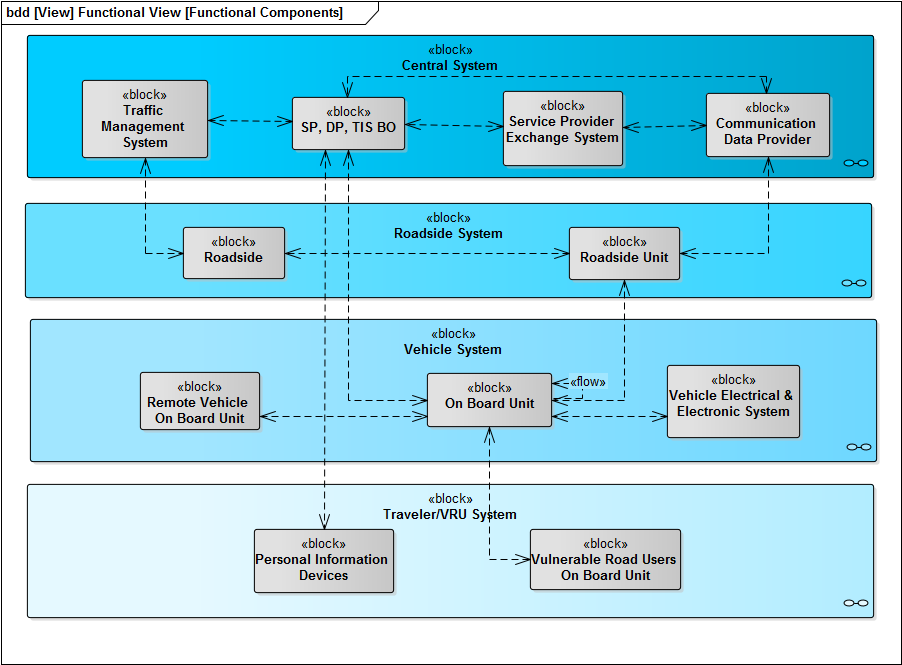
\includegraphics[width=0.45\textwidth]{functional}
	\caption{Functional Model Representation of the C-MobILE Reference Architecture}
	\label{fig:functional}
	\centering
\end{figure}

A functional viewpoint in the abstract level describes the system's runtime functional elements and primary interactions\cite{sysml}. The functional view (Figure \ref{fig:functional}) conforms to the functional viewpoint, helps the system's stakeholders understand the system structure, and has an impact on the system's quality properties.

As discussed previously, the systems were further decomposed into subsystems. The subsystems are depicted in the Functional model in Figure \ref{fig:functional} as functional elements with primary interaction with other subsystems. 

The subsystems for the Central System are:

\begin{itemize}
	 \item the Traffic Management System (TMS):
	 A functional back-office system of the responsible road operator to enforce legal actions on the roads
	 \item SP/DP/TIS BO: 
	 Generic Back-Office systems for Service Providers and Data Providers that collects and fuses date from service providers, vehicles and infrastructure
	 \item Service Provider Exchange System (SPES): 
	 An e-Market system for discovery and exchange of ITS services
	 \item Communication Data Provider: 
	 A generic back-office system of a communication provider user for access at several communication systems from other BO systems).
\end{itemize}

The subsystems for the Roadside System are:
\begin{itemize}
	\item Roadside: Different types of existing systems such as a Traffic Light controller or substations
	\item Roadside Unit: A cooperative roadside communication system responsible for two-way communication functionality at a part of a road network.
\end{itemize} 

The subsystems for the Vehicle System are:
\begin{itemize}
	\item On Board Unit (OBU): A sub-system attached to a car and needed for informing/advising the driver through a HMI 
	\item Remote Vehicle On Board Unit: An OBU of the other vehicle that is communication with the host vehicle
	\item Vehicle Electrical \& Electronic System: The parts of the vehicle such as in-car light sensors, speed sensors and actuators).
\end{itemize} 

The subsystems for the Traveler/VRU System are:
\begin{itemize}
	\item  Personal Information Devices (PID): Typically a smartphone or personal navigation device used by an end-user
	\item Vulnerable Road Users On Board Unit: An OBU attached to a VRU vehicle like bicycle or moped and need to advices the cyclists or the moped driver.
\end{itemize} 




\section{Lessons Learned}
 As previously described there are various existing projects being deployed at the C-MobILE partner deployment sites. To consolidate these and come up with a C-Mobile C-ITS reference architecture was a challenge. To address these concerns and achieve the aim of the reference architecture we followed the following approach.
\begin{enumerate}
	\item We analyzed the existing projects and abstracted the commonalities.
	\item We had weekly architecture team meetings comprising of architecture expertise from the C-MobILE partner deployment sites and other C-ITS projects that helped us in aligning the knowledge and concepts required to structure the reference architecture.
	\item We adapted SysML as a modeling language to describe the architecture as it is a mature language that is known to majority of system architect. It being supported by many mature tools such as Enterprise Architect was helpful.
	\item Since there was no standardized architecture framework in any of the existing projects, we defined the architecture framework using the conceptual model of ISO/IEC/IEEE 42010 \cite{iso42010}. This helped us in defining the views and viewpoints that satisfies the concerns of the stakeholders participating in the C-MobILE project.
\end{enumerate}

\section{Conclusions and Further Work}

\todo{revisit the goals, we have analysed the ref. architecture and developed, compatible with ditcm and can be used in deployment sites}

We were able to cover and satisfy each of the selected C-ITS services.
\todo{conclusion}

In this paper we present the reference architecture defined for the C-MobILE project.
%In the C-MobILE project we analysed existing C-ITS architectures, especially CONVERGE, MOBiNET, and Dutch C-ITS Reference Architecture, to define common concepts and vocabulary for the C-MobILE reference, concrete, and implementation architectures.
%We used the different architectures from the deployment sites as an input for defining a single homogeneous reference architecture, which will be further refined.
%We employed a reverse architect approach for manually extracting components, systems, and technological details.
The next step is to automate this approach, with the intention to provide benefits for system architects and stakeholders.


\section*{Acknowledgments}

The C-MobILE project is funded by the European Union's Horizon 2020 research and innovation programme under grant agreement No 723311.


\begin{thebibliography}{00}

    \bibitem{ec} European Commission. Directive 2010/40/eu of the european parliament and of the council.
    \bibitem{ecits} European Commission. Intelligent transport systems. \url{https://ec.europa.eu/transport/themes/its/c-its_en}.
    \bibitem{ditcm} Sambeek, M.v., Ophelders, F., Bijlsma, T. and Kluit, B.v.d, Turetken, O., Eshuis, R., Traganos, K. and Grefen, P. Towards an architecture for cooperative-intelligent transport system (c-its) applications in the netherlands. Available at \url{ https://www.researchgate.net/publication/313580768_Towards_an_Architecture_for_Cooperative-Intelligent_Transport_System_C-ITS_Applications_in_the_Netherlands}.

	\bibitem{ditcmits} Passchier, I., Sambeek, M.v., Broek, J.v.d. and Potters, P. The Dutch C-ITS Reference architecture. Paper number EU-TP0105. 11th ITS European Congress, Glasgow, Scotland, 6-9 June 2016.

    \bibitem{iso42010} ISO/IEC/IEEE Systems and software engineering -- Architecture description," in ISO/IEC/IEEE 42010:2011(E) (Revision of ISO/IEC 42010:2007 and IEEE Std 1471-2000) , vol., no., pp.1-46, Dec. 1 2011 doi: 10.1109/IEEESTD.2011.6129467
    
    \bibitem{archframework}Emery, D., and Rich, H. Every architecture description needs a framework: Expressing architecture frameworks using ISO/IEC 42010. Software Architecture, 2009 \& European Conference on Software Architecture. WICSA/ECSA 2009. Joint Working IEEE/IFIP Conference on. IEEE, 2009.
    
    \bibitem{ITSCongress} Ferrandez, R., Dajsuren, Y., Karkhanis, P., Fünfrocken, M. Pillado, M. C-MobILE C-ITS Reference Architecture. ITS World Congress 2018 (in submission).
    \bibitem{c-its} Festag, A. "Cooperative intelligent transport systems standards in europe," in IEEE Communications Magazine, vol. 52, no. 12, pp. 166-172, December 2014.  doi: 10.1109/MCOM.2014.6979970
    
    \bibitem{itsbegin} Osório, A.L., Afsarmanesh, H. and Camarinha-Matos, L.M. Towards a reference architecture
    for a collaborative intelligent transport system infrastructure. In Luis M. Camarinha-Matos, Xavier Boucher, and Hamideh Afsarmanesh, editors, Collaborative Networks for a Sustainable
    World, pages 469–477, Berlin, Heidelberg, 2010. Springer Berlin Heidelberg.
    
    \bibitem{ivhs} Heermann, P.D. and Caskey, D.L. Intelligent vehicle highway system: Advanced public transportation
    systems. Mathematical and Computer Modelling, 22(4):445 – 453, 1995.
    
    \bibitem{prometheus} Williams. M. Prometheus-the european research programme for optimising the road transport
    system in europe. In IEE Colloquium on Driver Information, pages 1/1–1/9, Dec 1988.
    
    \bibitem{racs} Takada, K., Tanaka, Y., Igarashi, A. and Fujita, D. Road/automobile communication system
    (racs) and its economic effect. In Vehicle Navigation and Information Systems Conference,
    1989. Conference Record, pages A15–A21, Sept 1989.
    
    \bibitem{sysml} Rozanski, N. and Woods, E. Software systems architecture: working with stakeholders using viewpoints and perspectives. Addison-Wesley, 2011.
    
    \bibitem{dajsuren2015design} Dajsuren, Y. On the design of an architecture framework and quality evaluation for automotive software systems. 2015.
    
    \bibitem{d31} Dajsuren, Y., Karkhanis, P., Kadiogullary, D. and Fuenfrocken, M. C-MobILE D3.1 Reference Architecture. Available at \url{http://c-mobile.diviprojects.wpengine.com/wp-content/uploads/sites/19/2018/03/C-MobILE-D3.1-ReferenceArchitecture_v0.1.pdf}
  
\end{thebibliography}


\end{document}
